\documentclass[11pt]{jsarticle}%article??

\usepackage{../mypackage}
%\usepackage[top=10truemm,bottom=10truemm,left=15truemm,right=15truemm]{geometry}
\usepackage[]{multicol}

\usepackage{titlesec}

\titleformat*{\section}{\large\bfseries}
\titleformat*{\subsection}{\normalsize\bfseries}
\titleformat*{\subsubsection}{\normalsize\bfseries}

%
% ######## measure #########
% # mm = 1mm = 2.85pt      #
% # cm = 10mm = 28.5pt     #
% # in = 25.4mm = 72.27pt  #
% # pt = 0.35mm = 1pt      #
% # em = width of [M]      #
% # ex = height of [x]     #
% # zw = width of [Kanji]  #
% # zh = height of [Kanji] #
% ##########################
% ##################### Portrait Setting #########################
% # TOP = 1inch + ¥voffset + ¥topmargin + ¥headheight + ¥headsep #
% #     = 1inch + 0pt + 4pt + 20pt + 18pt (default)              #
% # BOTTOM = ¥paperheight - TOP -¥textheight                     #
% ################################################################
\setlength{\textheight}{\paperheight}   % 紙面縦幅を本文領域にする(BOTTOM=-TOP)
\setlength{\topmargin}{-5.4truemm}       % 上の余白を30mm(=1inch+4.6mm)に
\addtolength{\topmargin}{-\headheight}  % 
\addtolength{\topmargin}{-\headsep}     % ヘッダの分だけ本文領域を移動させる
\addtolength{\textheight}{-40truemm}    % 下の余白も30mm(BOTTOM=-TOPだから+TOP+30mm)
% #################### Landscape Setting #######################
% # LEFT = 1inch + ¥hoffset + ¥oddsidemargin (¥evensidemargin) #
% #      = 1inch + 0pt + 0pt                                   #
% # RIGHT = ¥paperwidth - LEFT - ¥textwidth                    #
% ##############################################################
\setlength{\textwidth}{\paperwidth}     % 紙面横幅を本文領域にする(RIGHT=-LEFT)
\setlength{\oddsidemargin}{-15.4truemm}  % 左の余白を25mm(=1inch-0.4mm)に
\setlength{\evensidemargin}{-15.4truemm} % 
\addtolength{\textwidth}{-25truemm}     % 右の余白も25mm(RIGHT=-LEFT)
%
%

\newif\iffigure
%\figurefaulse
\figuretrue
%select show the figure or not

\makeatletter
\def\@cite#1{\textsuperscript{#1)}}
\def\@biblabel#1{#1)}
\makeatother

\newcommand{\DATE}[3]{#1年#2月#3日} 
\newcommand{\TheDay}{\DATE{2020}{12}{01}}
\newcommand{\rHeader}{東京大学工学部航空宇宙工学科 中須賀・船瀬研究室}
\newcommand{\lHeader}{令和2年度学士論文}

%題名は重要そう 対話的とか入れたいかなあ←要らないと言われた
\title{衛星内の情報伝達経路モデルに基づく\\不具合分析支援に関する研究} 
\date{} %これ日付と名前が横配置にできないかを考える
\author{\TheDay ~~~~~ 03-183005 西本 慎吾}

%ヘッダの指定:
\pagestyle{fancy}

\begin{document}
%2段組みにする
\maketitle

%ここら辺のフォントを変えたい
\thispagestyle{fancy}
\lhead[\lHeader]{\lHeader} % ヘッダ左側
%\chead[偶数ページの引数]{奇数ページの引数} %ヘッダ中央
\rhead[\rHeader]{\rHeader} %ヘッダ右側
%\lfoot[偶数ページの引数]{奇数ページの引数} %フッタ左側
%\cfoot[偶数ページの引数]{奇数ページの引数} %フッタ中央
%\rfoot[偶数ページの引数]{奇数ページの引数} %フッタ右側

%\columnseprule=0.3mm

\begin{abstract}
  近年,大学や高専などの教育機関や,民間企業による超小型衛星の
開発,およびそれを利用した事業の展開が盛んになっている.
一方で,超小型衛星の信頼性の低さが問題となっている.%修正
軌道上故障に関する調査の結果
信頼性の低さの原因として,設計および製造過程における不良が多いことが分かっており,
地上試験によって不具合の改修,対策を十分に行うことが重要である.
 しかし,衛星のような複雑なシステムでは,
 一つの不具合事象に対して多くの故障が考えられ,不具合事象から
故障箇所の特定を行うことは非常に多くの知識と経験を必要とする. 
 そこで,本研究ではコンポーネント間の接続関係モデル,情報
 伝達経路モデルを用いて衛星の故障候補の検証手順(打つべきコマンド,確認事項)を探索し,
 それらをコマンドの安全性及び,故障候補切り分け能力を示す指標
 %人間の判断を支援する指標%この言い方が曖昧過ぎる
 と共に提示することで,
 不具合分析を支援する手法を提案する.
 本手法を用いて,簡易的な衛星モデルに対して不具合分析を実践することで, 
 コマンドによる故障箇所の特定作業が体系化できること,設計不備の発見%設計の不備という言い方はよくないかもしれない
 につながることを確認した.%確認していない
%多分背景以外のところをもう少し詳細に述べたほうがいい気がする.
\end{abstract}
%これはどうするか要検討
\begin{multicols}{2}
%もうちょい縮められるかも
\vspace{-12zh}
\begin{eqnarray*}
   &&\text{C} : \text{コマンド} \\
   &&\text{T} : \text{テレメトリ} \\
   &&l: \text{リンク(コンポーネント間の接続関係)}\\
   &&\text{R}: \text{経路}\\
   &&P(l_{i} = \text{normal}) : \text{リンク}l_i\text{の正常確率}\\
   &&\mathbb{F}: \text{経路R内の故障候補リンクの集合}\\
   &&\mathbf{N_F}: \text{コマンドが形成する経路内の故障候補リンクの数}\\
\end{eqnarray*}
\vspace{-6zh}
  \section{序論}
  \vspace{-1zh}
  \subsection{研究背景}
  \vspace{-1zh}
  超小型衛星開発に大学などの参加が増加している中,
  信頼性の低さが問題となっている\cite{Langer2016}.
  軌道上故障の調査の結果,衛星の故障原因の多くは設計・製造過程にある\cite{Venturini2017}
  ことが分かっており,それらの多くは地上試験によって確認することができるものである
  という調査結果が出ている\cite{SAITO2011}.
  \vspace{-1zh}
  %設計・製造における不良が軌道上故障の多くを占めている現状がある.
  %解決するためには地上試験において,設計上の不良を発見し十分に改修しなけらばならない.
  \begin{figure}[H]
    \centering
      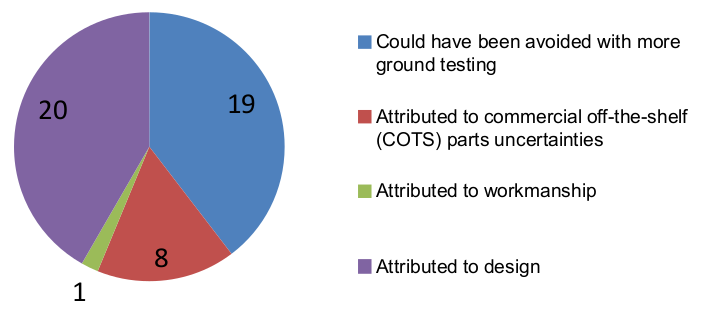
\includegraphics[height=3.0cm]{../figure/cause_of_failure.png}
      \caption{超小型衛星の故障原因に関する調査結果\cite{Venturini2017}}
      \label{fig:cause_of_failure}
  \end{figure}
  
 % \vspace{-1zh}
  %地上試験の不備が発生する原因として地上試験で改修を行う難しさがあるということを言いたい
  \subsection{問題提起}
  \vspace{-1zh}
  以上より,地上試験での不具合分析が不十分になっていることが,超小型衛星の
  信頼性の低さの原因の一つである.地上試験での不具合分析を十分に行うためには
  以下の2点の作業に高い知識と経験が必要とされる.
  %地上試験における検証が不十分になっている原因の一つとして故障候補の洗い出しや故障箇所の
 %特定作業が知識依存になっていることが挙げられる.
  \begin{itemize}
    \item 故障仮説の生成
    \item 故障候補の検証%検証としたほうがいい??
  \end{itemize}
  まず,故障仮説の生成はFTA(Fault Tree Analysis)%これはどうなんや?
  などを用いて不具合事象から考えられる故障モード
  を網羅的に洗い出す.衛星は内部機器の物理的相互作用が複雑
  に絡み合っているため,人による思い付きでは網羅的に行うことは困難である.\\
  %アクティブセンシングを行うことを述べる.それが安全である必要がある
  また,故障候補の検証は衛星から得られる情報を元に
  衛星の安全を確保しながら行う必要がある.
  実ミッションで使用するコマンドとテレメトリは膨大な数であるため,
その中から切り分けを行うための情報を選択し,仮説の検証を行う作業は
無駄やヒューマンエラーを生むきっかけとなる.\\
これらの課題に対して,表\ref{tab:previous_research}に示すように,
故障候補の洗い出しを網羅的に行う研究が盛んにおこなわれている.
一方で,不具合分析の大きな課題の一つである検証過程に関して取り組んだものは少ない.
%一方で,故障候補の切り分ける過程に関して取り組んだ研究は少ない.
%安全に行う必要があることを言いたい.
\vspace{-1zh}
%比較軸が微妙過ぎる
\begin{table}[H]
  \centering
  \caption{不具合分析手法の比較}
  \label{tab:previous_research}
   \scalebox{0.8}{
     \begin{tabular}{cccccc} \hline%もう少し示し方を考える.
        手法&故障網羅性&手法の目的%&モデル複雑度%専門家の知識が必要という点で?
        \\ \hline
        GDE&低&故障仮説生成%&低
        \\ %見てないし無くてもいいかも
        GDE+\cite{Struss1989}&中&故障仮説生成%&中
        \\
        網状故障解析\cite{Yamaguchi2014}&中&異常モード洗い出し%&高
        \\
        故障オントロジー\cite{Kitamura1999}&高&故障仮説生成%&高
        %\\
        %本手法&中%低かもしれない.接続関係しか見れていない
        %&故障箇所特定支援%&中
        \\ \hline %本手法は入れないほうがいいのか..
     \end{tabular}}
\end{table}
\vspace{-1zh}
\subsection{本研究の目的}
\vspace{-1zh}
以上より,衛星の故障箇所を特定する作業を
体系化し,不具合分析経験の少ない人が十分に不具合分析を
行える様に支援することが必要である.
よって,本研究では以下の機能を満たす不具合分析支援手法の提案%何の手法か分からん
を目的とする.%システムを作ることではなくて手法を提案することにしたほうがきれい?
  \begin{itemize}
  %\item 異常テレメトリから故障候補を生成する.%ここはいらんかも
  \item 故障候補を確認するためのコマンドおよびテレメトリを提案する.
  \item コマンドを選ぶ際の判断の指標を定量的に提示する.
\end{itemize}
\vspace{-1zh}
\section{情報伝達経路モデルに基づく不具合分析支援手法}
\vspace{-1zh}
\subsection{手法の概要}
\vspace{-1zh}
上述した機能を実現するために,本手法は以下の要素から構成されている.
\begin{itemize} %ここの順番と以下の順番を一致させる
  \item 衛星内部機器の接続関係モデル及び情報伝達経路モデル
  \item 故障仮説検証の流れ及び検証用コマンドの探索アルゴリズム%これいるのか?説明する価値があるのか?
  \item コマンドの安全性及び,故障候補切り分け能力を示す指標
\end{itemize}
本手法を用いた不具合分析システムの構成を図\ref{fig:whole_flow}に示す.
本手法は人間と対話的に故障箇所の特定を行う.これにより %うむ,人間による推論も使える..
実機の情報をシステムに反映しながら故障箇所を絞り込むことができる.
%テレメトリの確認から始め,初期コマンド状態からの確認.という風にやっていくってところも欲しい
\begin{comment}
\begin{figure}[H]
  \centering
    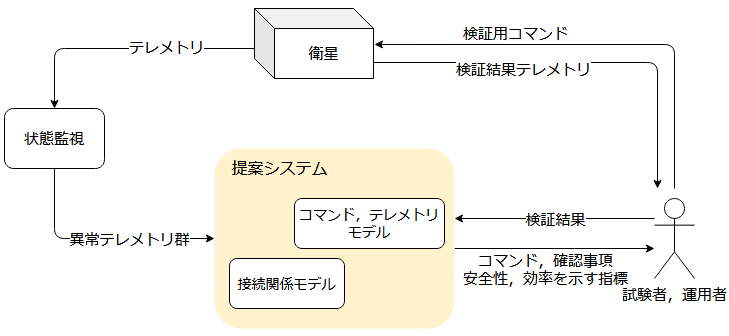
\includegraphics[width=8cm]{../figure/System_architect.png}
    \caption{提案手法の構成}
    \label{fig:System_architect}
\end{figure}
\end{comment}
%故障仮説の生成は研究対象ではないので,簡単に通る経路としていることも言ったほうがいい
\begin{figure}[H]
  \centering
    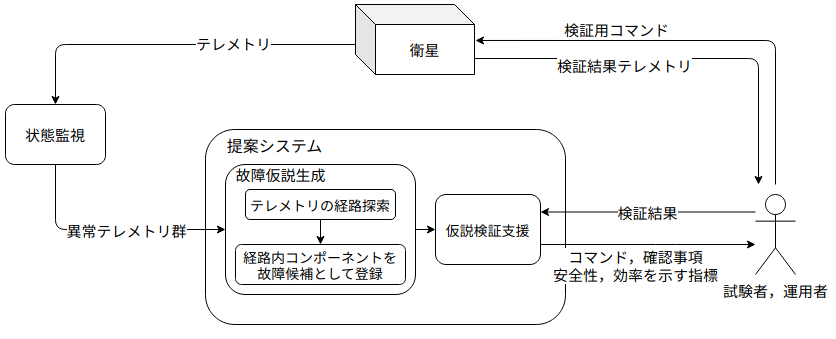
\includegraphics[width=7.0cm]{../figure/whole_flow.png}
    \caption{本手法による不具合分析の構成}
    \label{fig:whole_flow}
\end{figure}
\vspace{-1zh}
\subsection{モデル}
  \vspace{-1zh}
  本手法で用いる情報伝達経路モデルを作成するために必要な,
各モデルに関して以下に示す.
%結局これ機能の話と接続関係の話が混ざってるから適切な分類なのかはわからない
\subsubsection{コンポーネント間接続関係モデル}
來村ら\cite{Kitamura01}は拡張デバイスオントロジーとして,機器間の接続関係を
「ポート」と「導管」という概念を用いて表現している.
これを元に,コンポーネントの接続関係を表す「リンク」(表\ref{fig:link})を定義した.各リンクには正常確率
を属性として持ち,これを用いて後ほど述べるコマンドの故障候補切り分け能力を定量化している.
また,表\ref{fig:compo}のように各コンポーネントがリンクを属性として持ち,コマンドの情報伝達
で使用するリンク(コマンドリンク)とテレメトリの情報伝達で使用するリンク(テレメトリリンク)を区別している.
\begin{table}[H]
  \centering
  \caption{リンク定義}
  \label{fig:link}
\end{table}
\vspace{-3zh}
\begin{figure}[H]
  \centering
    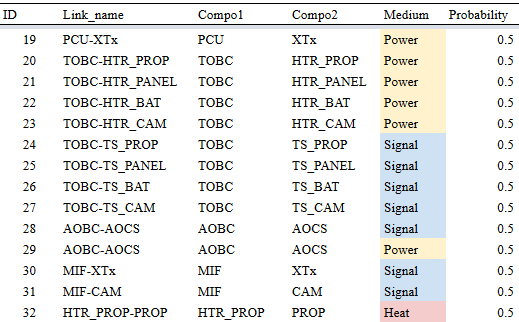
\includegraphics[height=5.0cm]{../figure/link_definition_resume.png}
\end{figure}
\vspace{-2zh}
\begin{table}[H]
  \centering
  \caption{コンポーネント定義}
  \label{fig:compo}
\end{table}
\vspace{-3zh}
\begin{figure}[H]
  \centering
    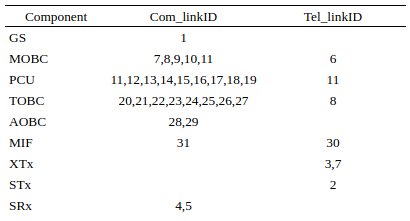
\includegraphics[height=3.5cm]{../figure/compo_link_resume.png}
\end{figure}
\vspace{-2zh}
%コマンド及びテレメトリのモデル→上記のモデルを用いることで衛星内部の情報伝達モデルを表現している的な
\subsubsection{情報伝達経路モデル}
  %次に,コマンドとテレメトリによる情報伝達経路のモデルに関して示す.
以下の表\ref{fig:COM},\ref{fig:TEL}のようにコマンドおよびテレメトリを定義した.
それぞれ情報伝達の経路を上述のリンクによって表現している.また,コマンドの属性として
「コマンド送信によって変化するテレメトリ」及び「種別」を定義している.
これらによって,コマンドが起こす状態変化
を表現し,内部状態の更新を行っている.%説明が曖昧過ぎる気がするな
%\vspace{-2zh}
\begin{table}[H]
  \centering
  \caption{コマンドモデル}
  \label{fig:COM}
\end{table}
\vspace{-3zh}
\begin{figure}[H]
  \centering
    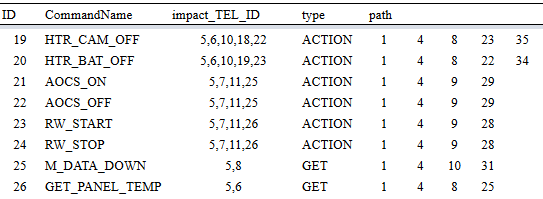
\includegraphics[width=8cm]{../figure/COM_resume.png}
\end{figure}
\vspace{-2zh}
\begin{table}[H]
  \centering
  \caption{テレメトリモデル}
  \label{fig:TEL}
\end{table}
\vspace{-3zh}
\begin{figure}[H]
  \centering
    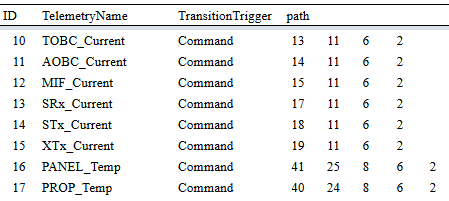
\includegraphics[height=3.5cm]{../figure/TEL_resume.png}
\end{figure}
\vspace{-1zh}
また,テレメトリのモデルでは,テレメトリに変化を及ぼすトリガの種類を指定しており,
これによって故障箇所特定に必要な情報取得のために取る行動を決めることができる.
ここでは簡単のため,軌道運動などによる状態変化は考慮せず,時間とコマンドによる
状態遷移のみを考えている.
\vspace{-1zh}
%論文側ではもう少し詳しく書く
\subsection{故障仮説検証の流れ}
\vspace{-1zh}
本手法によって故障仮説の検証を行う流れ及び検証用コマンド探索
のアルゴリズムを図\ref{fig:algorithm}に示す.
故障仮説の検証を行う流れとして,まずは取得済みテレメトリによって確認を行い,
その後コマンドによる確認に移る.この時,検証用コマンドの探索アルゴリズム
は図に示す通りで,コマンドとテレメトリによる経路が故障候補のリンクを通り,
そのコマンドによって発生する
状態変化があれば,故障候補を確認可能なコマンドとしている.%日本語
\vspace{-1zh}
%機能に関しては必要ないかもしれない.とりあえず必要なのはつながりと経路.
%それに確率があることを説明する
%コマンドおよびテレメトリの機能モデル%これは違うかも
%でも状態量の更新に関して説明するために必要.
%やっぱりこれいる気がする.何を持って確認するコマンド及びテレメトリと言えるのかがわからない
\begin{figure}[H]
  \centering
    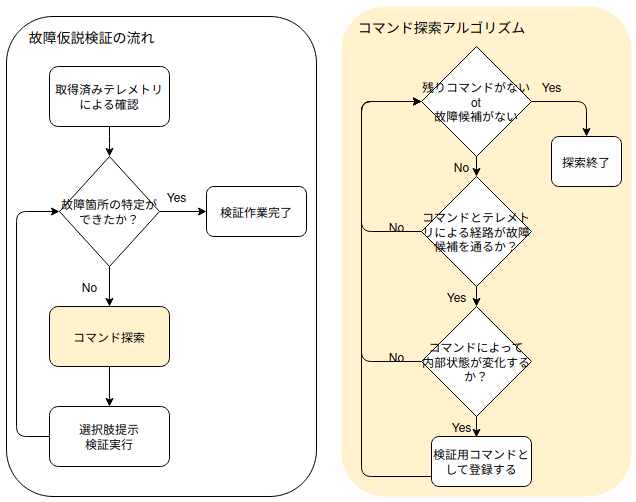
\includegraphics[height=5.5cm]{../figure/COM_search_algorithm.png}
    \caption{故障仮説検証の流れ及び検証用コマンド探索アルゴリズム}%短くしたいな
    \label{fig:algorithm}
\end{figure}
\vspace{-1zh}
\subsection{評価指標の提案}
  \vspace{-1zh}
  本手法の対象は地上試験における支援であるが,不具合分析に利用する情報の粒度が
コマンドとテレメトリのみであるため,軌道上不具合発生時の故障箇所特定にも
利用可能である.そこで,以下では地上試験及び軌道上での運用時の両方で重要となる
指標を提案し,本手法が両状況で使い分け可能な枠組みであることを示す.
\vspace{-1zh}
%なんでこの2点を指標にするのかを説明する.
  \subsubsection{コマンドの衛星生存性への副作用}
  まず,生存への副作用を示す指標として,以下の3点を与える.
\vspace{-1zh}
\begin{itemize}
    \item コマンドを打つ前の電力状態と,コマンドを打つことによって発生する電力消費量
    \item 姿勢変化を起こすか否か
    \item コマンド送信によって変化するテレメトリの数
  \end{itemize}
  前者2点の電力と姿勢の制約による指標は運用時に特有のものであり,コマンドを打つことで
  衛星の安全を脅かすことがないように危険な動作を明示的に示すことで,
  未熟な運用者による誤ったコマンド送信を防ぐ目的がある.
  また,不具合発生時は衛星の状態に対する把握が不十分であるため,衛星の状態を大きく変化
  させるコマンドは危険であるといえる.そのため,コマンドによって発生する状態変化
  の大きさを定量的に示す指標として3点目の指標を与えている.
\vspace{-1zh}
\subsubsection{コマンドの故障候補切り分け能力}
  運用時は可視時間が限られており,その時間内に不具合の改修を行わなければ
  ミッション失敗につながるような,時間制約を考慮した不具合分析を行う場面が考えられる.
  その際には,少ないコマンド数で効率的に故障箇所の特定を行えることが望ましい.
  以下ではコマンドの切り分け能力として,一つのコマンドによる切り分け能力を示す指標と
  全体の効率を考えた指標に関して示す.
  %ここが余り繋がってないように思える.

 まず,一つのコマンドで確認できる故障候補の数を表す指標に関して述べる.
 %この図は使っているようで使えていない
 %一つのコマンドに対して複数の経路ができること,それに応じて結果が変化することを言ったほうがいい
 以下の図\ref{fig:route}の例に示すように,あるコマンドC$_k$によって
 形成される経路が複数存在する場合を考える.%3つでなくてもいい
 あるリンク$l_i$の状態を確認するためにはその経路$\text{R}_j$内にある他のリンク
 が正常である必要があるため,$l_i$を確認できる確率は式(\ref{eq:P l R})となる.
 \begin{eqnarray}
  P(l_{i} | \text{R}_j) &=& \prod_{m\in\mathbb{F}_j,i\neq m} P(l_{m} = \text{normal})
  \label{eq:P l R}
\end{eqnarray}
 %ここで$\mathbb{F}_j$は$\text{R}_j$内の故障候補
 %リンクの集合,$P(l_{m} = \text{normal})$は上述した各リンクの正常確率を表している.
 また,$P(l_{i} | \text{R}_j)$はコマンドが形成する各径路すべてに対して求まるので
 それらの最大値を取りコマンドC$_k$による$l_i$の確認可能性は式(\ref{eq:P l C})となる.
 %これの式にkがないのがダメとか言われそう
\begin{eqnarray}
  P(l_i|\text{C}_k) &=& \max  \{ P(l_i|\text{R}_{j_k})\} \label{eq:P l C}
\end{eqnarray}
\vspace{-1zh}
\begin{figure}[H]
  \centering
     \begin{tabular}{c}
        \begin{minipage}{0.30\hsize}
        \centering
        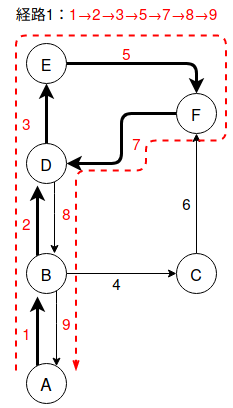
\includegraphics[height=4.5cm]{../figure/route1.png}
         %  \caption{}
           \label{fig:route1}
        \end{minipage}
        \begin{minipage}{0.30\hsize}
        \centering
        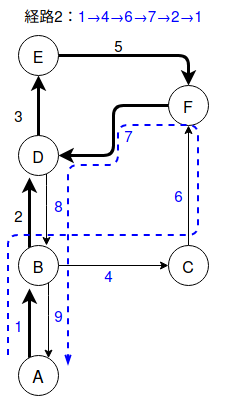
\includegraphics[height=4.5cm]{../figure/route2.png}
        %\caption{}
           \label{fig:route2}
        \end{minipage}
        \begin{minipage}{0.30\hsize}
           \centering
           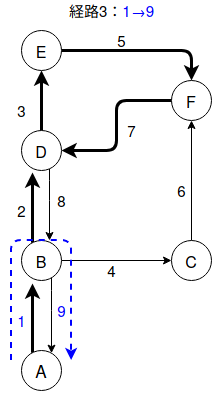
\includegraphics[height=4.5cm]{../figure/route3.png}
           %\caption{}
              \label{fig:route2}
           \end{minipage}
     \end{tabular} 
     \caption{故障候補(太矢印)と検証用コマンドC$_1$による情報伝達経路の例}%ここも変えたほうがいいかも
     \label{fig:route}
\end{figure}
\vspace{-1zh}
また,式(\ref{eq:P l C})が各リンクに対して求められるのでそれらの平均である
「平均確認可能性$P_m(\text{C}_k)$」,
及びC$_k$によって確認可能なリンクの数を表す「確認可能リンク数$E(\text{C}_k)$」
が以下のように求まる.
%ここで,$\mathbf{N_{F_k}}$はコマンドが形成する経路内にある全ての故障候補の数を表す.
\begin{eqnarray}
  P_m(\text{C}_k) &=& \frac{1}{\mathbf{N_{F_k}}}\sum_{i=1}^{\mathbf{N_{F_k}}}
  P(l_i|\text{C}_k) \label{eq:Pm Ck} \\
  E(\text{C}_k) &=& \mathbf{N_{F_k}}P_m(\text{C}_k) =
   \sum_{i=1}^{\mathbf{N_{F_k}}}P(l_i|\text{C}_k) \label{eq:E Ck}
\end{eqnarray}
%図がどこに入るかでスペースを調整する必要がある.
式(\ref{eq:Pm Ck}),(\ref{eq:E Ck})がどちらも高いコマンドを選択することで,
一つのコマンドでより多くの故障候補の状態を確認することが可能である.

次に,あるコマンドから検証を開始した時に,最終的に故障箇所の特定を行うまでにかかる
コマンドの総数に関して述べる.
図\ref{fig:all_process}に示すように,あるコマンドによる検証を考えると
各テレメトリの結果によって検証結果が異なる.この時,故障候補が残っている場合には
それに応じたコマンドの探索を行う必要がある.そのため,図\ref{fig:all_process}に示す
各Caseそれぞれで,最終的に故障箇所を特定するまでのコマンドの総数が異なる.\\
各テレメトリが正常値を示すか否かは各リンクごとの正常確率を用いて式(\ref{eq:P_TEL_normal}),
(\ref{eq:P_TEL_abnormal})のように算出でき,これを元に図\ref{fig:all_process}の各Caseになる確率が求まる.
%各Caseになる確率は
%検証のために使用するコマンドの数を見積もることができる.
%この図は論文の流れがないとわけわからない.
%スライドで上手く説明したいが,一度abnormalになったときは次にnormalとなることはないという仮定をしている
\vspace{-1zh}
\begin{figure}[H]
  \centering
    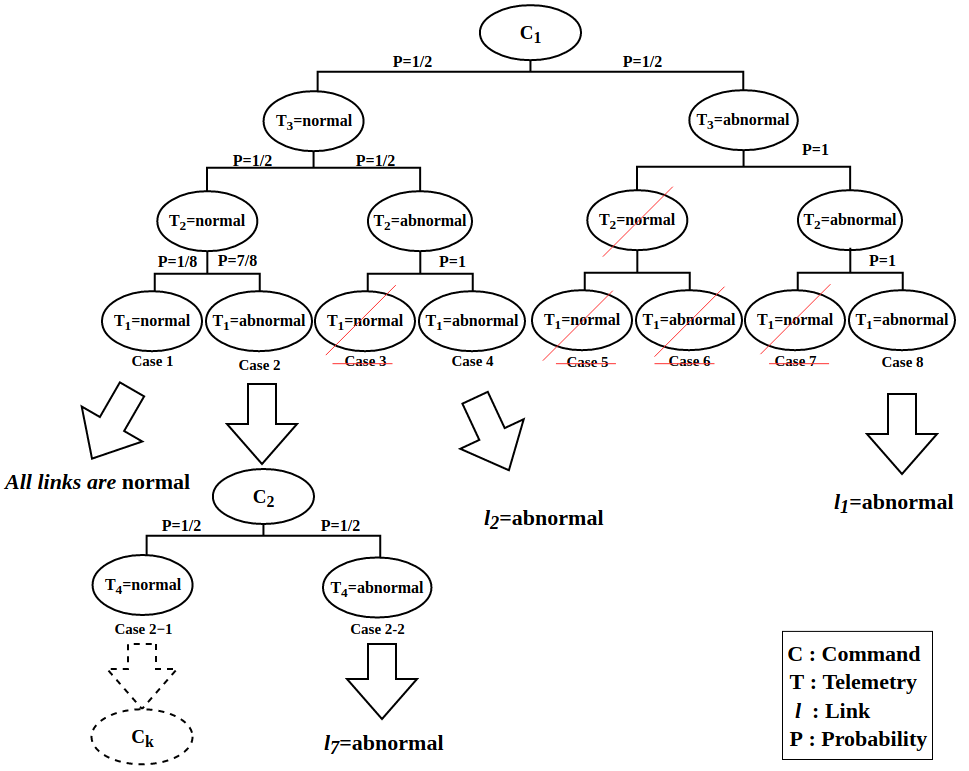
\includegraphics[height=6.5cm]{../figure/all_process.png}
    \caption{検証プロセスの全体像(テレメトリのIDは図\ref{fig:route}の経路と対応)}
    \label{fig:all_process}
\end{figure}
\vspace{-1zh}
%ここで,$\text{T}_j$はIDが$j$のテレメトリを表しており,経路(R$_j$)の添え字と対応している.
\begin{eqnarray}
  P(\text{T}_j = \text{normal}) &=& \prod_{i\in\mathbb{F}_j} P(l_i = \text{normal}) \label{eq:P_TEL_normal}\\
  P(\text{T}_j = \text{abnormal}) &=& 1 - P(\text{T}_j = \text{normal}) \label{eq:P_TEL_abnormal}
\end{eqnarray}
また,テレメトリの結果の組み合わせによって,各Caseになる確率$P(\text{Case }i)$が求められる.
これを用いて式(\ref{eq:N Ck})のように検証にかかるコマンド数の期待値が求められ,
これを「検証コマンド総数」と定義する.
ここで,$\mathbb{C}$は検証が終了した結果の各場合(Case)の集合である.%日本語が変かも
%P(Case i)に関しては表式がめんどくさすぎるので書かない
\begin{eqnarray}
  N(\text{C}_k) &=& \sum_{\text{Case }i\in\mathbb{C}} P(\text{Case }i) N_{\text{Case }i} \label{eq:N Ck}
\end{eqnarray}
検証コマンド総数が少ないコマンドを選択することによって,全体的に
かかるコマンドの数の期待値が小さい検証プロセスを選択することができ,時間制約を考えた場合に
重要な指標であると言える.
\vspace{-1zh}
\subsubsection{評価指標の使い分け}
%安全重視のときは何で,効率重視のときは何なのかを話すべき.
%その後に地上試験は電力姿勢を考えなくていいことを話す
まず,安全重視で故障候補の切り分けを行う場合は,
電力及び姿勢を考慮し,コマンド送信によって変化するテレメトリの数が少ないコマンドを
選択すれば良い.
また,効率重視で故障候補の切り分けを行う場合は,
平均確認可能性及び確認可能リンク数が高く,
検証コマンド総数が小さいコマンドを選択すれば良い.\\
%一方でではない気がする
この時,切り分け能力の高いコマンドは同時に,「変化するテレメトリの数」が多く
なる傾向にあるので効率と安全性を両立させることは難しく,
トレードオフを考えて選択する必要がある. %これいるかな?
%運用時のような時間制約を考える場合には$N(\text{C}_k)$を最優先するべき?

また,地上試験において電力や姿勢が制約になることはないため,考慮する必要はない.
%表の残骸
\begin{comment} 
\begin{table}[H]
  \centering %高,中,低の方がいいかも
  \caption{地上試験と運用時での指標の優先度(\textcolor{red}{赤}:安全重視,黒:効率重視)}
  \label{tab:indicator usage}
  \scalebox{0.8}{
    \begin{tabular}{c|ccc|cccc} \hline %段作って効果と副作用に分けたほうがいいかも
      &電力&姿勢&影響TEL数&$P_m(\text{C}_k)$&$E(\text{C}_k)$&$N(\text{C}_k)$ \\ \hline
      地上試験&-&-&\textcolor{red}{高},低&\textcolor{red}{低},高&\textcolor{red}{低},高&\textcolor{red}{低},高\\
      運用時&\textcolor{red}{高},低&\textcolor{red}{高},低&\textcolor{red}{高},低&\textcolor{red}{低},高&\textcolor{red}{低},高&\textcolor{red}{低},高\\ \hline
    \end{tabular}}
\end{table}
\end{comment}
\vspace{-1zh}
\section{本手法による不具合分析の実践と評価}
  \vspace{-1zh}
  \subsection{問題設定}
  \vspace{-1zh}
  以下の図\ref{fig:satellite}のような構成の簡易的な衛星のモデルを対象にし
  以下の2つの故障状態の例に対し,本手法を用いた不具合分析を実践した.
 %温度計故障に関しては減らすかもしれない
  \begin{itemize}
   \item ヒータの接触不良
   \item 温度計故障(断線)
 \end{itemize}
 %図の記号が何を表しているかを説明入れたい.口頭で?
  \begin{figure}[H]
    \centering
      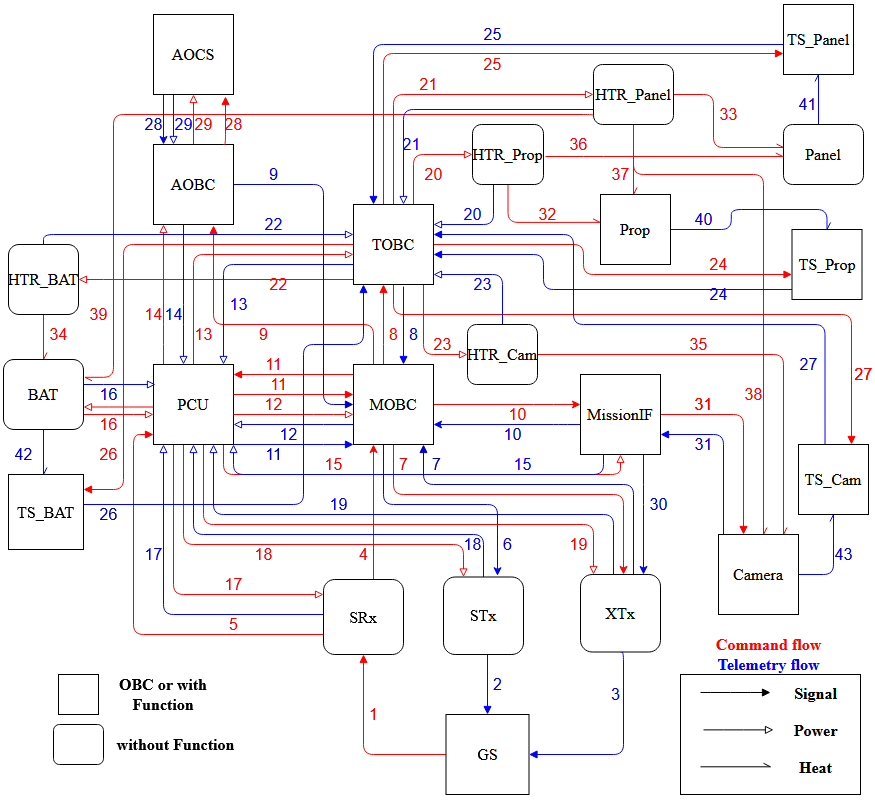
\includegraphics[height=7.5cm]{../figure/satellite_diagram.png}
      \caption{衛星内コンポーネント接続関係図(数字はリンクのID)}
      \label{fig:satellite}
  \end{figure}
\vspace{-1zh}
\subsection{実践結果}
  \vspace{-1zh}
  \subsubsection{ヒータの接触不良}
  %\vspace{-1zh}
図\ref{fig:satellite}に示す,推進系ヒータ(HTR\_PROP)と推進系(PROP)の間(ID:32)
の故障を考える.
%多分この図要らない.アルゴリズムとして説明する?
\begin{comment}
  \begin{figure}[H]
    \centering
      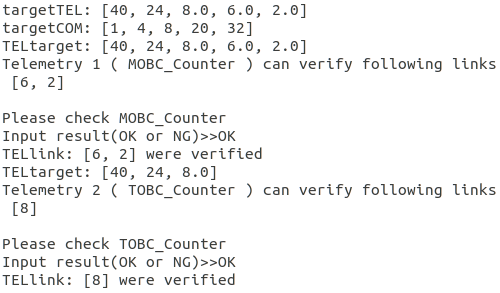
\includegraphics[width=6.0cm]{../figure/COM14_TEL17_TEL_phase.png}
      \caption{テレメトリによる確認事項の提示}
      \label{fig:TEL_list}
  \end{figure}
  \vspace{-1zh}
  \begin{figure}[H]
    \centering
      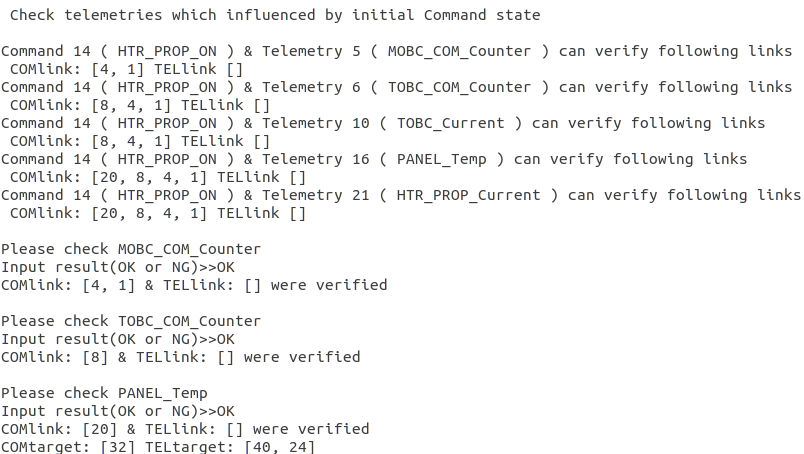
\includegraphics[width=8.0cm]{../figure/COM14_TEL17_iniCOM_phase.png}
      \caption{初期コマンドを用いた確認}
      \label{fig:initial_COM}
  \end{figure}
\end{comment}  
この時,現れる不具合事象は「推進系ヒータONコマンドを送った時,推進系温度が変化しない」
である.
%ここで説明するべきか検討.ここじゃ伝わらんよな
本手法では,不具合発生時のコンポーネントの状態として,
送信したコマンドによって変化した後の
状態になっていると仮定して,初期状態を与えている.\\
%かつヒータの状態もパネルはOFFになっているとか色々あるが,上手く表現できないか?
上述した不具合分析の流れに従って,取得テレメトリでの切り分けから行い,
検証用コマンドの探索した結果が図\ref{fig:COM_candidate}のようになる.
  %この図を可視化したものにできると嬉しい
  %提示された選択肢だけをコンソール画面で表示.絞り込んでいくプロセスはグラフで
 \begin{figure}[H]
   \centering
     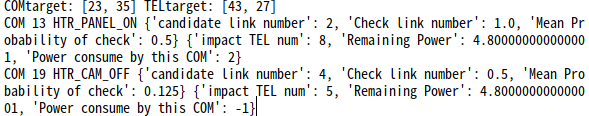
\includegraphics[width=8.0cm]{../figure/COM_candidate.png}
     \caption{検証用コマンド探索結果}
     \label{fig:COM_candidate}%出力結果に数式の記号使う
 \end{figure}
%各指標の対応付けを言ったほうがいいかもしれない.提示されている文字が何を意味するのか分からない
%これも推進系ヒータONというふうに日本語で言うべき?
%状態変化を起こすものを対象にしている.
選択肢として,パネルヒータON(13:HTR\_PANEL\_ON)と推進系ヒータOFF(18:HTR\_PROP\_OFF)
が提示されており,どちらから選択しても図\ref{fig:COM_process}のように,故障箇所
の特定ができた.
\begin{figure}[H]
  \centering
    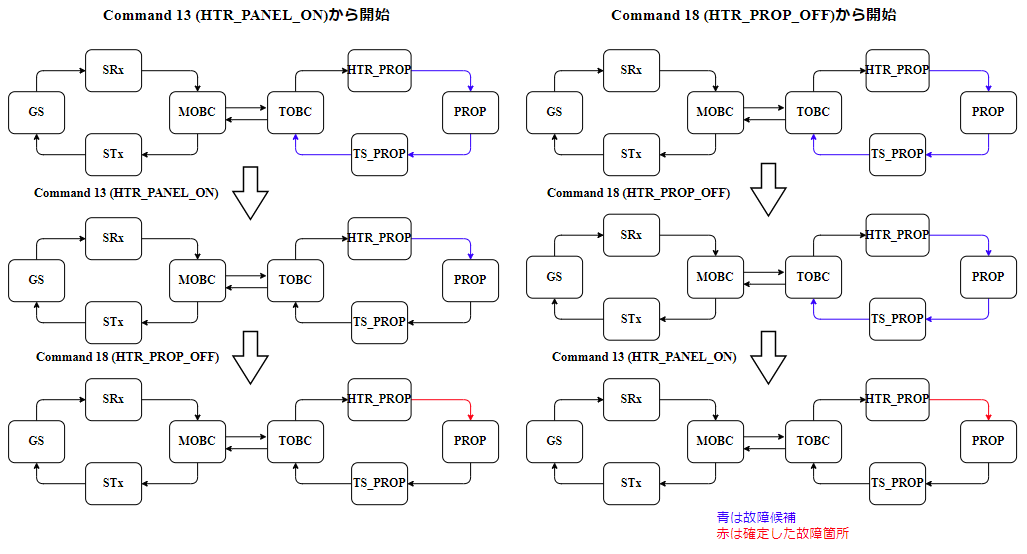
\includegraphics[width=8.0cm]{../figure/COM_process_HTR_PROP_fault.png}
    \caption{ヒータ接触不良時の検証プロセスによる違い}
    \label{fig:COM_process}
\end{figure}
%このやり方が人が行うものと何が違うのか?
%どこが正しくて何が違うのか?→実際は上の不具合時ヒータがONになっているかはわからないので
%OFFが状態を変えるコマンドとしているのが違う.
\subsubsection{コマンドの指標に関する考察}
図\ref{fig:COM_process}に示したように,コマンドの選択順序によって切り分けを行う過程に
違いが見られた.
まず,平均確認可能性(図\ref{fig:COM_candidate}中のPm(C))が高い
「パネルヒータON」から検証を行ったほうが一つ目のコマンドで大きく
絞り込めている.
%後でここをやる
%「パネルヒータON」から検証した場合,初めに「PROP-TS\_Prop間」,「TS\_Prop-TOBC間」%ここも日本語の方が好ましい?
%の正常が確認でき,1つのコマンドで残り1つのリンクにまで絞り込めている.\\%びみょいな
%最終的に「HTR\_Prop-PROP間」の異常を確認して故障箇所を特定している.\\
一方で,「推進系ヒータOFF」から検証した場合は1つ目の検証では故障候補を切り分けることができず,
2つ目のコマンド「パネルヒータON」によって推進系温度の上昇を確認できるため,
「PROP-TS\_Prop間」,「TS\_Prop-TOBC間」の正常が確認できている.\\
運用時,通信が不安定であり不具合分析に使える時間が明確でない時は,
一度のコマンドで多くの確認ができることが望ましいため,図\ref{fig:COM_process}の左側のように
平均確認可能性が高いコマンドから検証を行うことで,1度のコマンド送信により,多くの絞り込みが
できる可能性が高いと言える.
%検証コマンド総数は最後まで検証を行うことを前提としていることを述べたいが,,,
\vspace{-1zh}
\subsubsection{本手法と人間の不具合分析の違い}
%ここもう少しコンパクトにできる
上で示した不具合事象「推進系ヒータONコマンドを送った時,推進系温度が変化しない」
に関して,同様の条件を与えて不具合分析を行う際の過程(送信するコマンド,コマンドを選択する理由,
確認するテレメトリ)を,本研究室の方々に対して調査した.%企業での経験がある人もいるよ

調査結果によると,多くの人が本手法での検証プロセスと同様な手順でコマンドの選択を行っており,
人間の推論と近い形で検証用のコマンドを探索できていることが分かる.
%言いたいのは以下.この安全性の評価ができていないことも言いたい
一方で,コマンドを選択した理由によると「推進系ヒータOFF」コマンドを選択するのは
故障可能性のあるコンポーネントによって二次故障の発生を防ぐために用いている.
%言い回しの問題
安全のために選択した「推進系ヒータOFF」コマンドによって切り分けられる故障候補も存在し,
確認事項を明示的に提示してくれるところが本手法の強みであると言える.
\vspace{-1zh}
\subsubsection{温度計故障}
最後に,推進系温度計の断線(テレメトリリンク24)に対する実践例を示す.
不具合事象としては上と同じものが考えられ,検証用コマンドの探索結果も同様になる.
温度計故障時の検証プロセスを以下の図\ref{fig:COM_phase_TS}に示す.
%この図なくしてもいいかもしれない
\begin{figure}[H]
  \centering
    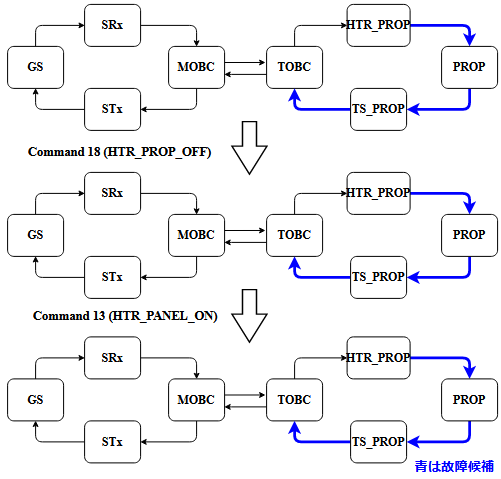
\includegraphics[width=6.0cm]{../figure/COM_process_TS_fault.png}
    \caption{温度計故障時の検証結果}
    \label{fig:COM_phase_TS}
\end{figure}
温度計の故障では,推進系への熱の伝わりを読み取る経路が1本しか無い
ため,熱の伝わりを観測することができす,本システムのみでは
故障箇所の特定を行うことができなかった.\\
%ここ上手く説明しないとやばい
一方で,不具合検証のプロセスで得た情報と人間による推論の組み合わせによって,
故障候補を絞り込むことは可能である.まず
取得テレメトリ「パネル温度」の上昇を確認できれば推進系ヒータが正常に動作していることが分かる.
また,「パネルヒータON」による推進系温度の変化が確認できなければ,
故障箇所が確実に「PROP-TS\_Prop間」,「TS\_Prop-TOBC間」の中に存在する
ことが分かる.\\
このように,提示された選択肢に従って検証を行うことで,故障箇所の推論に必要な
情報を得ることができる.また,人間の推論を組み合わせても故障箇所の特定が
行えなかった場合には,設計の不備を考えることができ,設計の正しさを確認するためにも利用できる.
\vspace{-1zh}
\section{結論}
\vspace{-1zh}
%やるべき優先順位としては,まとめのところで目的と対応が取れているかと,新規性に関してしっかりと
%主張ができているかというところ
\subsection{まとめ}
\vspace{-1zh}
本研究では,衛星の情報伝達経路モデルを用いてコマンドによる故障箇所特定の過程を
体系化する手法,及びコマンドの安全性と故障候補切り分け能力の大きさを示す指標
を提案し,テストケースで実践した.\\
実践例では,複数のコマンドの中から故障箇所特定のために適切なコマンドを提示し,
想定した故障箇所を特定できることを示した.
次に,提案した指標に基づいてコマンドを選択することで時間制約の厳しい不具合分析
の際に効果的な分析が行える可能性があることを示した.
%もう少し人との推論で特定できる,そのための情報を効率的に集めることができることを伝える.
また,システムのみでは特定を行えなかった場合も,
人間の推論と組み合わせることで故障候補の絞り込みができ,
提示された選択肢に従うことで推論に必要な情報を効率的に得ることができることが分かった.

%ここの順番を考える.
%最後の否定を人間との比較からつなげる?
一方で,本手法で見ることができる故障は主に接続関係に起因するものであり,
コンポーネントが持つ機能の故障まで特定することはできない.
%テレメトリを発行している機器の故障の場合は,そのコンポーネントから
%の情報ラインに冗長系がなければかなり多くの故障候補が残ってしまう.
%多分複数の検証結果を総合して判断するような処理が必要になるんやろな.これをシステム上で判断させること
%ができれば実現できるのかもしれないが,ムズいぜ
\vspace{-1zh} 
\subsection{今後の課題}
\vspace{-1zh} 
今後以下の様な課題に取り組む必要があると考えている.
\begin{itemize}
  \item コンポーネントの機能の接続関係を組み込んだ,より粒度の細かい故障箇所特定
  \item リンクの正常確率に実機の情報を組み込むことによる,検証の効率化
  \item 設計情報からのモデル自動生成
  %\item コマンドの安全性の評価・・・
  %\item 推論も
\end{itemize}

\begin{comment}
  
今後,接続関係の異常だけでなく,実問題に近い故障状態も扱えるようにするために,
 扱う状態量をより詳細にモデル化していく必要がある.また,テレメトリと状態量の対応付けを考えることによって
 異常状態をリンクとして表現するのではなく,各コンポーネントの機能の異常を特定できると考えている.

 %???
検証結果の入力形態として,正常か異常の2値だけ,定性的なパラメータを入力できる様に拡張して
行く必要があると考えている.

正常か異常かの判断は人に依存してしまっている.


 リンクの正常確率として,より実機で用いているコンポーネントの信頼度に近い値を考えることで,
 モデルが複雑になった際により効率的な故障箇所特定を行えると考えている.

 最後に,本研究において使用したモデルは手作業にて構築したが,
 実ミッションでの適用を考慮すると手作業によるモデル化は人為的ミスや,コストを考えると現実的ではない.
 今後,設計情報などから必要な情報を抽出してモデルを自動生成できるように工夫する必要があると考えている.
\end{comment}

  
  \bibliographystyle{junsrt} %plain, acm, alpha とか
  \bibliography{../Ref} 

\end{multicols}
\end{document}